\documentclass[cjk,dvipdfm,12pt,%
hyperref={bookmarks=true,bookmarksnumberd=true,bookmarksopen=false,%
colorlinks=false,%
pdftitle={Debian GNU/kFreeBSD$B$GJk$i$;$k4D6-$r9=C[$7$F$_$k(B},%
pdfauthor={$B?yK\E5=<(B},%
pdfinstitute={dictoss@live.jp},%
pdfsubject={$BBh(B38$B2s4X@>(BDebian$BJY6/2q(B},%
}]{beamer}

\title{Debian GNU/kFreeBSD$B$GJk$i$;$k4D6-$r9=C[$7$F$_$k(B}
\subtitle{{\scriptsize{$\sim$$BBh(B38$B2s4X@>(BDebian$BJY6/2q(B$\sim$}}}
\author[$B?yK\(B $BE5=<(B]{{\large\bf $B?yK\E5=<(B}}
\institute[]{{\normalsize\tt dictoss@live.jp}}
\date{{\small 2010 $BG/(B 8 $B7n(B 22 $BF|(B}}

%\usepackage{amsmath}
%\usepackage{amssymb}
\usepackage{graphicx}
\usepackage[varg]{txfonts}
%\usepackage{D6math}
\AtBeginDvi{\special{pdf:tounicode EUC-UCS2}}
\usetheme{Kyoto}
\def\museincludegraphics{%
  \begingroup
  \catcode`\|=0
  \catcode`\\=12
  \catcode`\#=12
  \includegraphics[width=0.9\textwidth]}
%\renewcommand{\familydefault}{\sfdefault}
%\renewcommand{\kanjifamilydefault}{\sfdefault}
\begin{document}
\settitleslide
\begin{frame}
\titlepage
\end{frame}
\setdefaultslide


\begin{frame}[fragile]
\frametitle{$BH/I=$K$*$$$F(B}
\begin{itemize}
  \item $B2?$+<ALd!"5?Ld$,$"$l$P?o;~<ALd$r$I$&$>!#(B
  \item $B%D%C%3%_!"Bg4?7^!#4V0c$$$r;XE&$7$F$$$?$@$/$H$3$N>l$N3'$5$s$,(B
$B9,$;$K$J$l$^$9!#(B
\end{itemize}
\end{frame}


\begin{frame}[fragile]
\frametitle{$B%"%8%'%s%@(B}
\begin{itemize}
  \item $B<+8J>R2p(B
  \item Debian GNU/kFreeBSD$B$H$O(B
  \item Debian GNU/kFreeBSD$B$N4D6-9=C[(B
  \begin{itemize}
    \item $B%$%s%9%H!<%k(B
    \item $B%+!<%M%k$N99?7(B
    \item xorg$B!"%G%9%/%H%C%W4D6-(B
    \item $BF|K\8l4D6-(B
    \item $B3+H/4D6-(B
    \item $B%G%P%$%9%I%i%$%P$NF3F~(B
  \end{itemize}
  \item $B=*$o$j$K(B
  \item $B<ALd%3!<%J!<(B
\end{itemize}
\end{frame}


\begin{frame}[fragile]
\frametitle{$BH/I=<T$K$D$$$F(B}
\begin{itemize}
  \item $BL>A0!'?yK\!!E5=<(B (dictoss@live.jp)
  \item Twitter : dictoss
  \item Debian GNU/Linux$B$OBg3X(B2$BG/$N:"$+$i;H$C$F$$$k!#(B
($BEv;~$O(Btesting$B$N(Bsarge)
  \item $B$3$3?tG/(BDebian GNU/Linux$B$H(BFreeBSD$B$r=8Cf$7$F;H$C$F$$$k!#(B
  \item Debian GNU/kFreeBSD$B$H$$$&?@(BOS$B$,9_NW$7$F$-$?$3$H$rCN$j!"(B
$B;H$$;O$a$?$N$,:rG/!#(B
\end{itemize}
\end{frame}


\begin{frame}[fragile]
\frametitle{Debian GNU/kFreeBSD$B$H$O(B}
\begin{itemize}
  \item Debian Project$B$G3+H/$,?J$s$G$$$k?7$7$$(BOS$B!#(B
  \item $B%+!<%M%k$O(BFreeBSD$B%+!<%M%k$r;HMQ!#(B
  \item $B%Q%C%1!<%8%7%9%F%`$O(Bdpkg/apt$B!#(B
  \item $B:NMQ%=%U%H%&%'%"$O(BDFSG$B$K=>$C$F7hDj$9$k!#(B
  \item $B8=CJ3,$G$O(Bi386$BHG$H(Bamd64$BHG$N(B2$B$D$N%"!<%-%F%/%A%c$r%5%]!<%H!#(B
  \item $B<g$J>pJs$O(BDebian Wiki$B$K$"$k!#(B($B1Q8l$J$N$G$+$s$P$C$FFI$_$^$7$g$&!#(B)
\end{itemize}
\end{frame}


\begin{frame}[fragile]
\frametitle{Debian GNU/kFreeBSD$B$H(BDebian GNU/Linux$B$N0c$$(B(1)}
\begin{itemize}
\item $B%G%P%$%9%I%i%$%P7O(B
  \begin{itemize}
  \item $B%5%&%s%I%G%P%$%9$O(BOSS$B!#(B
  \item eth0$B$OB8:_$7$^$;$s!#(B($B$3$N%^%7%s$O(Bem0$B$GG'<1$7$F$$$^$9(B)
  \item $B%G%#%9%/%G%P%$%9L>$O!V(B/dev/ad4s1$B!W(B($BFbB"(BHDD)$B$d(B
$B!V(B/dev/da0s1$B!W(B(USB$B%a%b%j(B)$B$H$7$FG'<1$9$k!#(B
  \item mount$B7O%3%^%s%I$,(B/sbin$B$N2<$K$?$/$5$s$"$C$?$j!"(B
$B%*%W%7%g%s$,<c430[$J$j$^$9!#(B
  \end{itemize}
\end{itemize}
\end{frame}


\begin{frame}[fragile]
\frametitle{Debian GNU/kFreeBSD$B$H(BDebian GNU/Linux$B$N0c$$(B(2)}
\begin{itemize}
\item $B%U%!%$%k%7%9%F%`7O(B
  \begin{itemize}
  \item $B8=;~E@$G$O(BUFS$B!"(Bext2$B$,;HMQ2DG=!#(B
  \item ext3$B$OFI$_9~$_$N$_2DG=!#(B
  \item $B:rF|(BDebian Wiki$B$r3NG'$7$?$i!"(Bzfsutils$B$H$$$&%Q%C%1!<%8$,DI2C$5$l$F!"(BZFS$B$,;H$($k$h$&$K$J$C$?LOMM!#(B(/$B%Q!<%F%#%7%g%s$r(BZFS$B$K$G$-$k$+$OITL@!#(B)
  \end{itemize}
\end{itemize}
\end{frame}


\begin{frame}[fragile]
\frametitle{Debian GNU/kFreeBSD$B$H(BDebian GNU/Linux$B$N0c$$(B(3)}
\begin{itemize}
\item $B2>A[2=(B
  \begin{itemize}
  \item FreeBSD$B$H$$$($P(BJail$B!#(B(chroot$B$N3HD%$G$9!#(B)
  \item VirtualBox (Debian$B%Q%C%1!<%8$H$7$F$"$k$,!&!&!&!#(B)
  \item QEMU
  \end{itemize}
\end{itemize}
\end{frame}


\begin{frame}[fragile]
\frametitle{$B%$%s%9%H!<%k(B}
\begin{itemize}
  \item $B%$%s%9%H!<%i$O(Bdaily$B%S%k%I$,$"$k$N$G%@%&%s%m!<%I$9$k!#(B
  \item $B:#2s$O(Bi386$BHG$r%$%s%9%H!<%k$7$^$7$?!#(B
\end{itemize}
\begin{center}
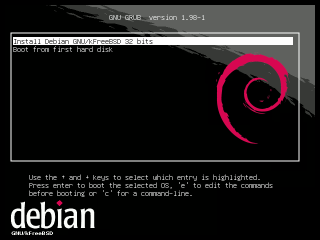
\includegraphics[scale=0.5]{image201008/kfreebsd-installer.png}
\end{center}
\end{frame}


\begin{frame}[fragile]
\frametitle{$B%+!<%M%k$N99?7(B(1)}
\begin{commandline}
$ uname -a
GNU/kFreeBSD deb-NorTP60 7.3-1-686 #0
Tue Jul 20 02:12:21 CEST 2010 i686 i386
Genuine Intel(R) CPU           T2400  @ 1.83GHz GNU/kFreeBSD
\end{commandline}
\begin{commandline}
$ cat /proc/cpuinfo
processor   : 0
vendor_id   : GenuineIntel
cpu family  : 6
model       : 7
model name  : Genuine Intel(R) CPU           T2400  @ 1.83GHz
stepping    : 8
flags       : fpu vme de pse tsc msr pae mce cx8 apic sep mtrr pge mca
              cmov pat b19 b21 mmxext mmx fxsr xmm b26 b27 b28 b29 3dnow
cpu MHz     : 1828.76
bogomips    : 1828.76
\end{commandline}
$B%$%s%9%H!<%kD>8e$O(BCPU$B$,(B1$B8D$7$+G'<1$7$F$$$J$$!#(B
\end{frame}


\begin{frame}[fragile]
\frametitle{$B%+!<%M%k$N99?7(B(2)}
\begin{commandline}
$ apt-cache search kfreebsd-image-*
kfreebsd-image-7-486 - kernel of FreeBSD 7 image
kfreebsd-image-7-686-smp - kernel of FreeBSD 7 image
kfreebsd-image-7-686 - kernel of FreeBSD 7 image
kfreebsd-image-7.3-1-486 - kernel of FreeBSD 7.3 image
kfreebsd-image-7.3-1-686-smp - kernel of FreeBSD 7.3 image
kfreebsd-image-7.3-1-686 - kernel of FreeBSD 7.3 image
kfreebsd-image-8-486 - kernel of FreeBSD 8 image
kfreebsd-image-8-686-smp - kernel of FreeBSD 8 image
kfreebsd-image-8-686 - kernel of FreeBSD 8 image
kfreebsd-image-8.0-1-486 - kernel of FreeBSD 8.0 image
kfreebsd-image-8.0-1-686-smp - kernel of FreeBSD 8.0 image
kfreebsd-image-8.0-1-686 - kernel of FreeBSD 8.0
\end{commandline}
\begin{commandline}
$ sudo apt-get install kfreebsd-image-7.3-1.686-smp
$ sudo reboot
\end{commandline}
\end{frame}


\begin{frame}[fragile]
\frametitle{$B%+!<%M%k$N99?7(B(3)}
\begin{commandline}
$ uname -a
GNU/kFreeBSD deb-NorTP60 7.3-1-686-smp #0
Tue Jul 20 02:43:20 CEST 2010 i686 i386
Genuine Intel(R) CPU           T2400  @ 1.83GHz GNU/kFreeBSD
\end{commandline}
\begin{commandline}
$ cat /proc/cpuinfo
processor   : 0
vendor_id   : GenuineIntel
model name  : Genuine Intel(R) CPU           T2400  @ 1.83GHz
processor   : 1
vendor_id   : GenuineIntel
model name  : Genuine Intel(R) CPU           T2400  @ 1.83GHz
stepping    : 8
flags       : fpu vme de pse tsc msr pae mce cx8 apic sep mtrr pge mca
              cmov pat b19 b21 mmxext mmx fxsr xmm b26 b27 b28 b29 3dnow
\end{commandline}
CPU$B$,(B2$B8D;H$($k$h$&$K$J$j$^$7$?!#(B
\end{frame}


\begin{frame}[fragile]
\frametitle{Xorg}
\begin{commandline}
$ sudo apt-get install xorg
Setting up hal (0.5.14-3) ...
Reloading system message bus config...
Failed to open connection to ``system'' message bus:
Failed to connect to socket /var/run/dbus/system_bus_socket: Connection refused
invoke-rc.d: initscript dbus, action ``force-reload'' failed.
Starting Hardware abstraction layer: haldinvoke-rc.d: initscript hal,
action ``start'' failed.
dpkg: error processing hal (--configure):
 subprocess installed post-installation script returned error exit status 1
\end{commandline}

$B$I$&$d$i4{CN%P%0$NLOMM$GL$2r7h>uBV!#(B

http://bugs.debian.org/cgi-bin/bugreport.cgi?bug=469528
\end{frame}


\begin{frame}[fragile]
\frametitle{Xorg}
\begin{itemize}
  \item $B860x$O(Bhal$B$N8e=hM}$G<B9T$9$k!V(B/etc/init.d/dbus reload$B!W$G%(%i!<$,(B
$BH/@8$7$?LOMM!#(B
  \item dbus$B$,Dd;_$7$F$$$k$N$G!V(B/etc/init.d/dbus start$B!W$G5/F0$7$?!#(B
  \item $B:FEY!V(Bapt-get install xorg$B!W!#(B
  \item $B$^$?<:GT$7$?$,>/$7?J$s$@$N$G!":FEY!V(B/etc/init.d/dbus start$B!W!#(B
  \item $B$H$j$"$($:(Bxorg$B$r%$%s%9%H!<%k$G$-$?!#(B
  \item xorg.conf$B$,$J$$$N$G?75,$K@8@.$7$F!"(B/etc/X11/xorg.conf$B$KG[CV!#(B
  \item startx$B$b@.8y$7$?$N$G$H$j$"$($:(BOK$B$H$9$k!#(B
\end{itemize}
\end{frame}

\begin{frame}[fragile]
\frametitle{gdm}
\begin{itemize}
  \item $B%$%s%9%H!<%k<+BN$O@.8y!#(B
  \item $B:F5/F0$9$k$H%-!<%\!<%IF~NO$,$G$-$J$$!*!*(B
  \item $B;EJ}$,$J$$$N$G(Bgdm$B$G$N%m%0%$%s$OD|$a$k!#(B
  \item gdm$B$N(Bpurge$B$K0l6lO+!#(B
\end{itemize}
\end{frame}

\begin{frame}[fragile]
\frametitle{$B%G%9%/%H%C%W4D6-(B}
\begin{commandline}
$ sudo apt-get install xfce4 xfce4-goodies
\end{commandline}

\begin{commandline}
$ vim ~/.xinitrc
exec xfce4-session

$ chmod 744 ~/.xinitrc
$ startx
\end{commandline}

$BL5;v$K(BXfce4$B$,5/F0$G$-$?!#(B
\end{frame}

\begin{frame}[fragile]
\frametitle{$BF|K\8l4D6-(B}
\begin{commandline}
$ sudo apt-get install otf-ipafont otf-ipaexfnt
$ sudo apt-get install locales-all
$ sudo apt-get install uim uim-anthy
\end{commandline}

\begin{commandline}
$ vim ~/.xinitrc
export LANGUAGE='ja_JP.UTF-8'
export LC_ALL='ja_JP.UTF-8'
export LANG='ja_JP.UTF-8'

export XMODIFIRES='@im=uim'
export GTK_IM_MODULE='uim'
export QT_IM_MODULE='uim'

exec xfce4-session

$ startx
\end{commandline}

$BF|K\8l$NI=<(!"F~NO$OLdBj$J$/2DG=$G$9!#(B
\end{frame}

\begin{frame}[fragile]
\frametitle{$B3+H/4D6-(B}
\begin{commandline}
$ sudo apt-get install gcc  g++ gdb make
$ sudo apt-get install build-essential pbuilder debian-keyring
\end{commandline}

$B;n$7$K(Btcsh$B$r%S%k%I$7$F$_$k!#(B
\begin{commandline}
$ apt-get source tcsh
$ sudo apt-get build-dep tcsh
$ cd tcsh-6.17.00
$ dch
$ debuild -i -us -uc -b
$ sudo dpkg -i tcsh_6.17.00-3.1_kfreebsd-i386.deb
\end{commandline}

deb$B%Q%C%1!<%8$N%S%k%I!"%$%s%9%H!<%k$,$G$-$^$7$?!#(B
\end{frame}

\begin{frame}[fragile]
\frametitle{Debian$BJY6/2q;qNA$N%S%k%I4D6-(B(1)}
\begin{itemize}
  \item contrib, non-free$B$N%Q%C%1!<%8$,I,MW$J$?$a!"(Bapt-line$B$r=$@5!#(B
\end{itemize}
\begin{commandline}
$ sudo vim /etc/apt/sources.list
deb http://ftp.jp.debian.org/debian/ squeeze main contrib non-free
deb-src http://ftp.jp.debian.org/debian/ squeeze main contrib non-free

deb http://security.debian.org/ squeeze/updates main
deb-src http://security.debian.org/ squeeze/updates main
\end{commandline}
\begin{commandline}
$ sudo apt-get install git-core
$ sudo apt-get install gs gs-esp gs-cjk-resource
$ sudo apt-get install ptex-bin xdvik-ja dvipsk-ja
$ sudo apt-get install okumura-clsfiles vfdata-morisawa5
$ sudo apt-get install texlive-latex-extra
$ sudo apt-get install poppler-data
$ sudo apt-get install evince
\end{commandline}
\end{frame}


\begin{frame}[fragile]
\frametitle{Debian$BJY6/2q;qNA$N%S%k%I4D6-(B(2)}
\begin{commandline}
$ cd
$ git clone git://git.debian.org/git/tokyodebian/monthly-report.git/
$ cd monthly-report
$ make
\end{commandline}
\end{frame}


\begin{frame}[fragile]
\frametitle{$BF|>o@83h$KI,MW$J%=%U%H%&%'%"$N%$%s%9%H!<%k(B}
\begin{commandline}
$ sudo apt-get install emacs emacs23-el
$ sudo apt-get install sylpheed sylpheed-i18n
$ sudo apt-get install iceweasel iceweasel-l10n-ja
$ sudo apt-get install audacious audacity
$ sudo apt-get install gxine
$ sudo apt-get install jd
$ sudo apt-get install gftp
\end{commandline}
\end{frame}

\begin{frame}[fragile]
\frametitle{$B%5%&%s%I%I%i%$%P$N%m!<%I(B(1)}
mp3$B$N%5%&%s%I%U%!%$%k$r:F@8$9$k$,2;$,LD$i$J$$!&!&!&!#(B

$B%5%&%s%I%I%i%$%P$r3NG'$7!"%m!<%I$7$^$9!#(B
\begin{commandline}
$ kldstat
 1   10 0xc0400000 890000   kfreebsd-7.3-1-686-smp.gz
 2    1 0xc0d9c000 57fdc    acpi.ko
 3    1 0xc5c7a000 67000    radeon.ko
 4    1 0xc5ce1000 14000    drm.ko
\end{commandline}
\begin{commandline}
$ sudo kldload snd_hda
$ kldstat
 1   10 0xc0400000 890000   kfreebsd-7.3-1-686-smp.gz
 2    1 0xc0d9c000 57fdc    acpi.ko
 3    1 0xc5c7a000 67000    radeon.ko
 4    1 0xc5ce1000 14000    drm.ko
 5    1 0xc611f000 1a000    snd_hda.ko
 6    1 0xc6139000 40000    sound.ko
\end{commandline}
\end{frame}

\begin{frame}[fragile]
\frametitle{$B%5%&%s%I%I%i%$%P$N%m!<%I(B(2)}
$B:F5/F0$9$k$H!"%5%&%s%I%I%i%$%P$,<+F0%m!<%I$5$l$J$$$N$G@_Dj$7$^$9!#(B

\begin{commandline}
$ sudo vim /etc/modules
# /etc/modules: kernel modules to load at boot time.
#
# This file should contain the names of kernel modules that are
# to be loaded at boot time, one per line.  Comments begin with
# a ``#'', and everything on the line after them is ignored.
snd_hda.ko
\end{commandline}

$B3F<o%+!<%M%k%b%8%e!<%k(B(*.ko)$B$O!"(B

/lib/modules/7.3-1-smp $B%G%#%l%/%H%j$N2<$K$"$j$^$9!#(B

$B!J(Bkfreebsd-image-7.3-1-smp$B$N%+!<%M%k$N>l9g!K(B
\end{frame}

\begin{frame}[fragile]
\frametitle{$B:#8e$N2]Bj(B}
\begin{itemize}
  \item Flash$B$N:F@84D6-(B
  \begin{itemize}
    \item Abobe$B8x<0$N(BFreeBSD$BHG%P%$%J%j$O$J$$!#(B
    \item $B:rF|;~E@$G(Bgnash$B$N%Q%C%1!<%8$,DI2C$5$l$F$$$?!#(B
$BF~$l$?$1$IF0$+$J$+$C$?$N$GF0$+$9J}K!$rC5$7$F$_$^$9!#(B
  \end{itemize}
  \item $B%S%G%*:F@8$NIJ<A$,0-$$!#(B(codec$B$+!)(B)
  \item Linux$B%P%$%J%j8_495!G=(B
  \item $B2>A[2=5!G=(B
  \item ZFS
\end{itemize}
\end{frame}

\begin{frame}[fragile]
\frametitle{$B4D6-9=C[$r=*$($F(B}
\begin{itemize}
  \item Debian$B%$%s%9%H!<%i$b@0Hw$5$l%$%s%9%H!<%k$7$d$9$$!#(B
  \item Debian GNU/kFreeBSD$B$b(BDebian GNU/Linux$B$bF1$8(BDebian$B$J$N$G>/$747$l$l$P(BOK$B!#(B
  \item $B$?$@!"F|$,@u$$(BOS$B$J$N$G%H%i%V%k$,5/$3$k$H(BFreeBSD$B%+!<%M%k$NLdBj$J$N$+!"(B
Debian$B%7%9%F%`$NLdBj$J$N$+!"@Z$jJ,$1$K;~4V$,$+$+$k!#(B
  \item BTS$B$O5.=E$J>pJs8;!#(B
  \item Debian GNU/kFreeBSD$B$O(BSqueeze$B$G5;=Q%W%l%S%e!<$H$7$F8x3+M=Dj!#(B
\end{itemize}
\end{frame}


\begin{frame}[fragile]
\frametitle{$B;29MJ88%(B}
\begin{itemize}
\item \url{http://tokyodebian.alioth.debian.org/pdf/debianmeetingresume201006-iwamatsu-presentation.pdf}
\item \url{http://wiki.debian.org/Debian_GNU/kFreeBSD_FAQ}
\end{itemize}
\end{frame}


\end{document}
%%% Local Variables: 
%%% mode: japanese-latex
%%% TeX-master: t
%%% End: 
